% vim: set tw=78 sts=2 sw=2 ts=8 aw et ai:
\documentclass{workshop}

% Comentează liniile de mai jos în cazul în care nu există cod de inclus.
\usepackage{code/highlight}
\usepackage{color}        % dacă e folosit highlight
\usepackage{alltt}        % dacă e folosit highlight
\usepackage{verbatim}
\usepackage{listings}

\title[Session 4]{Session 4}
\subtitle{Kernel Debugging}
\author{Daniel Băluţă, Irina Preşa}
\date{July 05, 2012}

\begin{document}

% Arătăm numărul frame-ului
\setbeamertemplate{footline}[frame number]

\frame{\titlepage}

% NB: Secțiunile nu sunt marcate vizual, ci doar apar în cuprins
\section{Printk}
\begin{frame}{Printk Loglevels}
Eight loglevels defined in $<$linux/kernel.h$>$ header.

\begin{itemize}
\item KERN\_EMERG: emergency messages, e.g. before a system crash.
\item KERN\_ALERT: serious problems that need a quick response.
\item KERN\_CRIT: critical condition, hardware or software failure.
\item KERN\_ERR: error conditions.
\item KERN\_WARNING: warning conditions.
\item KERN\_NOTICE: situations that require notification.
\item KERN\_INFO: info/log messages.
\item KERN\_DEBUG: debug phase only.
\end{itemize}
\end{frame}

\begin{frame}{Printk Loglevels}
\begin{itemize}
\item numbers from 0 to 7, smaller values are higher priorities.
\item by default is the level described by DEFAULT\_MESSAGE\_LOGLEVEL
variable.
\item klogd and syslogd display only the messages with priority less or equal
to DEFAULT\_CONSOLE\_LOGLEVEL.
\item the base priority can be changed with sys\_syslog syscall or by writing
to /proc/sys/kernel/printk.
\end{itemize}
\end{frame}

\begin{frame}{Printk Loglevels}
\begin{itemize}
\item printk writes messages in a circular buffer.
\item it wakes any processes that are waiting for messages.
\begin{itemize}
\item e.g. from the syslog syscall or a process that reads /proc/kmsg.
\end{itemize}
\item if the buffer fills up, it overwrites the old data.
\end{itemize}
\end{frame}

\section{Understand a Kernel Oops}
\begin{frame}{Understand a Kernel Oops}
\begin{figure}
  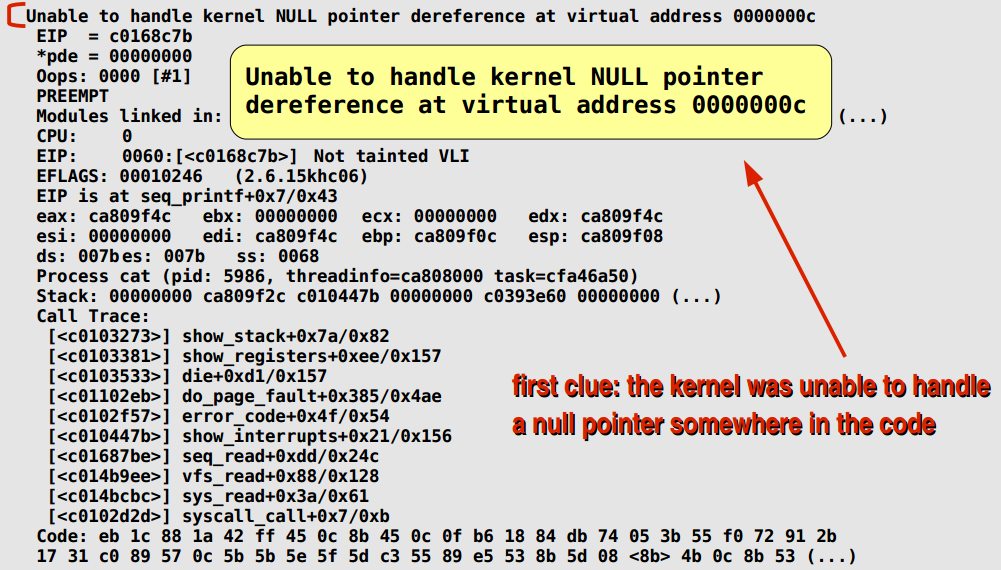
\includegraphics[scale=0.3]{img/1.png}
  \end{figure}
\end{frame}

\begin{frame}{Understand a Kernel Oops}
\begin{figure}
  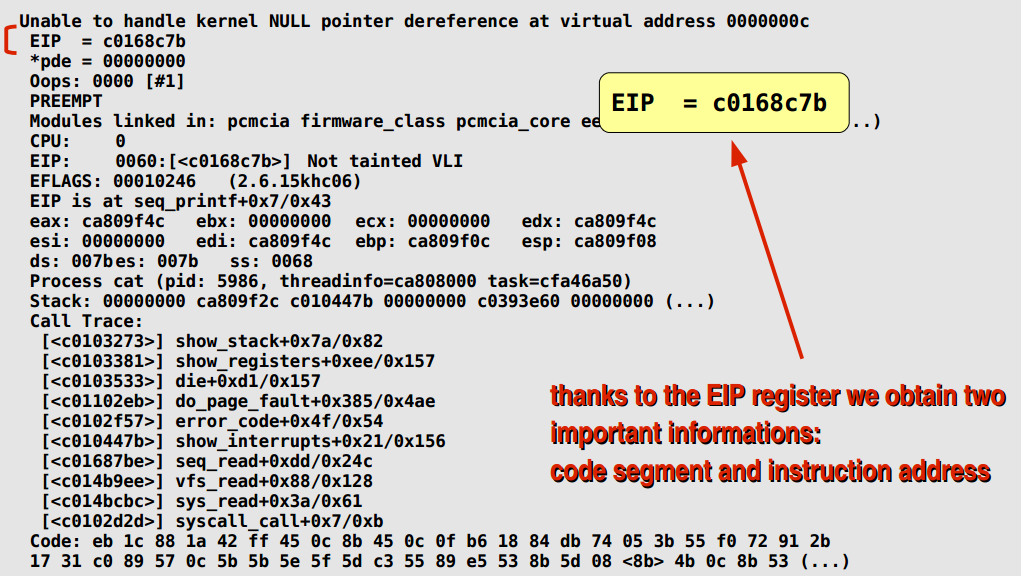
\includegraphics[scale=0.3]{img/2.png}
  \end{figure}
\end{frame}

\begin{frame}{Understand a Kernel Oops}
\begin{figure}
  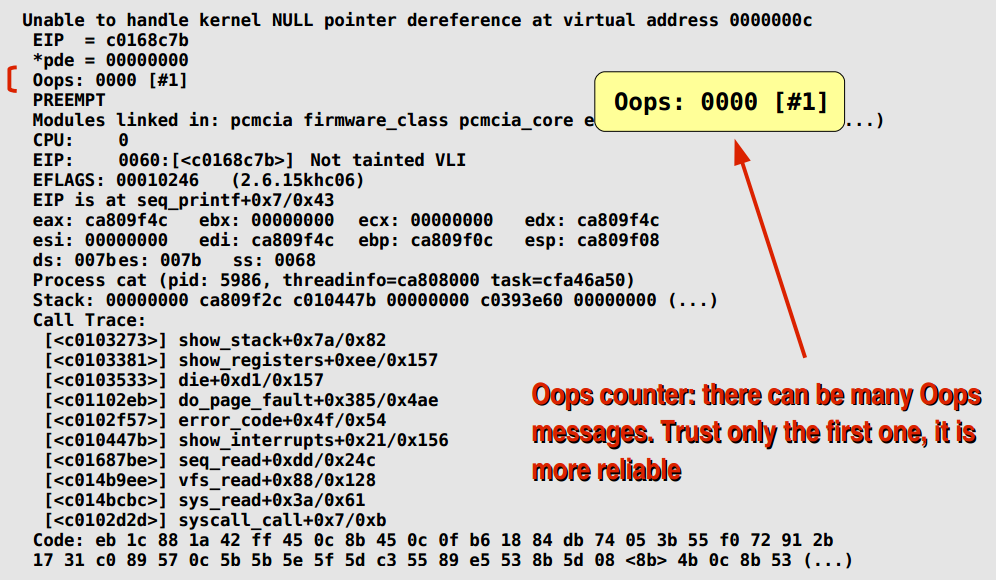
\includegraphics[scale=0.3]{img/3.png}
  \end{figure}
\end{frame}

\begin{frame}{Understand a Kernel Oops}
\begin{figure}
  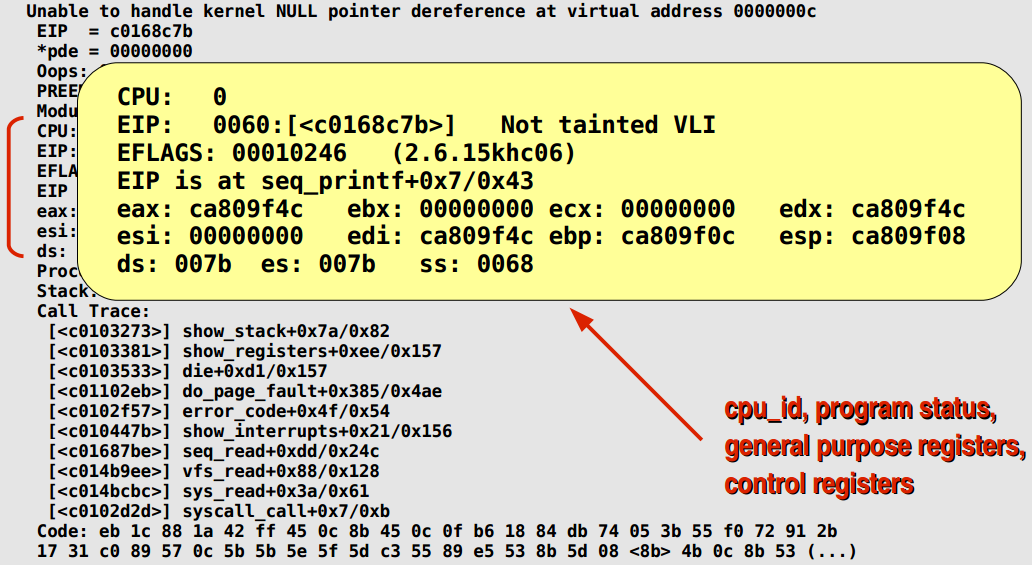
\includegraphics[scale=0.3]{img/5.png}
  \end{figure}
\end{frame}

\begin{frame}{Understand a Kernel Oops}
\begin{figure}
  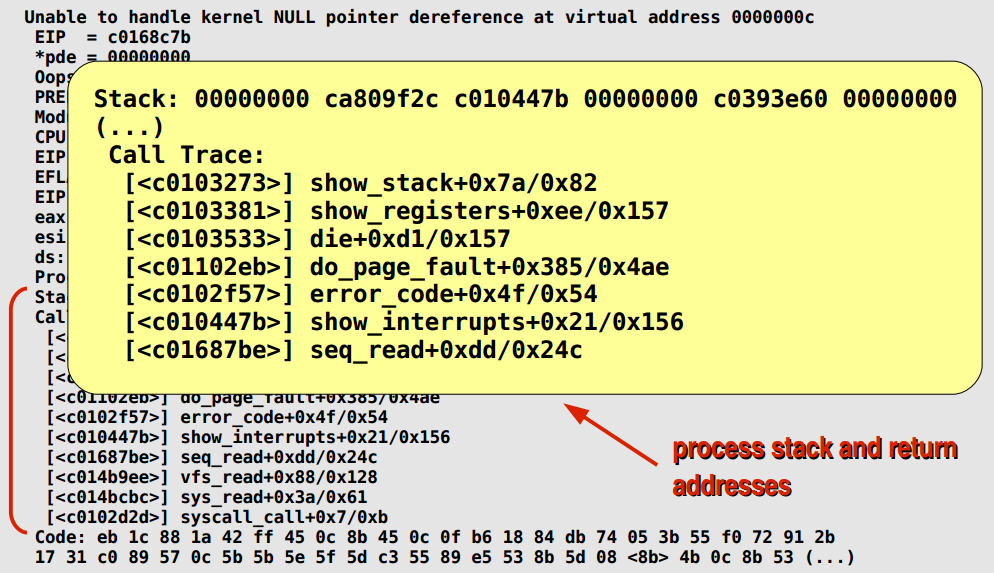
\includegraphics[scale=0.3]{img/6.png}
  \end{figure}
\end{frame}

\section{Classical Debug Solutions}
\begin{frame}{Classical Debug Solutions}
\begin{itemize}
\item Tools:
\begin{itemize}
\item objdump, addr2line
\item gdb, dump\_stack
\end{itemize}
\item Data:
\begin{itemize}
\item vmlinux, module objects
\item /proc/kcore, System.map
\end{itemize}
\end{itemize}
\end{frame}

\begin{frame}[fragile]{Addr2line}
\begin{verbatim}
Unable to handle kernel NULL pointer dereference
at virtual address 00000fc5 pgd = c5db8000
[00000fc5] *pgd=16aba031, *pte=00000000, *ppte=00000000
Internal error: Oops: 11 [#1] PREEMPT
last sysfs file: /sys/power/state
Modules linked in:
CPU: 0    Not tainted  (2.6.32 #385)
PC is at msmfb_suspend+0x1c/0x2c
LR is at msmfb_suspend+0x20/0x2c
pc : [<c01b063c>] lr : [<c01b0640>] psr: a0000013
\end{verbatim}

\begin{verbatim}
# arm-none-linux-gnueabi-addr2line -f -e vmlinux c01b063c
#/kernel/linux/drivers/video/msm/msm_fb.c:485
\end{verbatim}
\end{frame}

\section{Memory Debug}
\begin{frame}{kmemleak}
\begin{itemize}
\item follows allocations similar with a garbage collector
\item scan allocated memory and kernel stack for memory leaks
\item CONFIG_DEBUG_KMEMLEAK
\item trigger a memory scan
\begin{itemize}
\item echo scan \textgreater /sys/kernel/debug/kmemleak
\end{itemize}
\item clear all posible leaks
\begin{itemize}
\item echo clear \textgreater /sys/kernel/debug/kmemleak
\end{itemize}
\item read memory leaks
\begin{itemize}
\item cat /sys/kernel/debug/kmemleak
\end{itemize}
\end{itemize}

\end{frame}

\section{Tracepoints and Kprobe}
\begin{frame}{...}
\end{frame}

\section{Netconsole and Netcat}
\begin{frame}{...}
\end{frame}

\section{Keywords}
\begin{frame}{Keywords}
      \begin{itemize}
        \item x
      \end{itemize}
\end{frame}

\section{Resources}

\section{Questions}

\end{document}
